
\newcommand{\CLASSINPUTinnersidemargin}{1in}
\newcommand{\CLASSINPUToutersidemargin}{1in}
\newcommand{\CLASSINPUTbottomtextmargin}{1in}
\newcommand{\CLASSINPUTtoptextmargin}{1in}


\documentclass[conference, nofonttune, letterpaper, twocolumn, 12pt, english, final]{IEEEtran}
%\documentclass[journal, twocolumn, 12pt, english]{}
%\usepackage[top=.75in, bottom=.75in, left=1in, right=1in]{geometry}
\usepackage{graphicx}
\usepackage{algorithmic}
\usepackage{fancyheadings}
%\usepackage{vmargin}
\usepackage{babel}
%\setmarginsrb{1in}{1in}{1in}{1in}{0pt}{0mm}{0pt}{0mm}
\pagestyle{fancyplain}
%\fancyfoot[C]{Robotics Club at UCF}
%\cfoot[\fancyplain{\thepage}{}]   
%\pagenumbering{arabic}
%\cfoot[<Robotics Club at UCF>]{Robotics Club at UCF}
%\usepackage{float}

\hyphenation{op-tical net-works semi-conduc-tor}
%\addtolength{\headsep}{0.2in}
%\addtolength{\topmargin}{-0.2in}
\cfoot[\thesection]{Robotics Club at UCF}
\rfoot[\thesection]{\thepage}
%
% paper title
% can use linebreaks \\ within to get better formatting as desired
\title{Robotics Club at UCF: \\
       The Gray Goose}


\author{\IEEEauthorblockN{David Adams}
\IEEEauthorblockA{Team Captain\\
Software Lead\\
dadams@ist.ucf.edu}
\and
\IEEEauthorblockN{Jonathan Mohlenhoff}
\IEEEauthorblockA{Electrical Lead\\
jmohlenh@ist.ucf.edu}
\and
\IEEEauthorblockN{Jake Carr}
\IEEEauthorblockA{Mechanical Lead\\
jakec@knights.ucf.edu}
\and
\IEEEauthorblockN{Brandon Parmeter}
\IEEEauthorblockA{Electrical and Mechanical Tech\\
bparmeter@knights.ucf.edu}
\and
\IEEEauthorblockN{Andrew Watson}
\IEEEauthorblockA{Electrical and Software Tech\\
andrewwatson@knights.ucf.edu}
\and
\IEEEauthorblockN{Ouns Mouri}
\IEEEauthorblockA{Electrical and Software Tech\\
omouri@gmail.com}
\and
\IEEEauthorblockN{Daniel Barber}
\IEEEauthorblockA{Faculty Advisor\\
dbarber@ist.ucf.edu}
}
\begin{document}
\maketitle



\begin{figure}[h!]
\centering
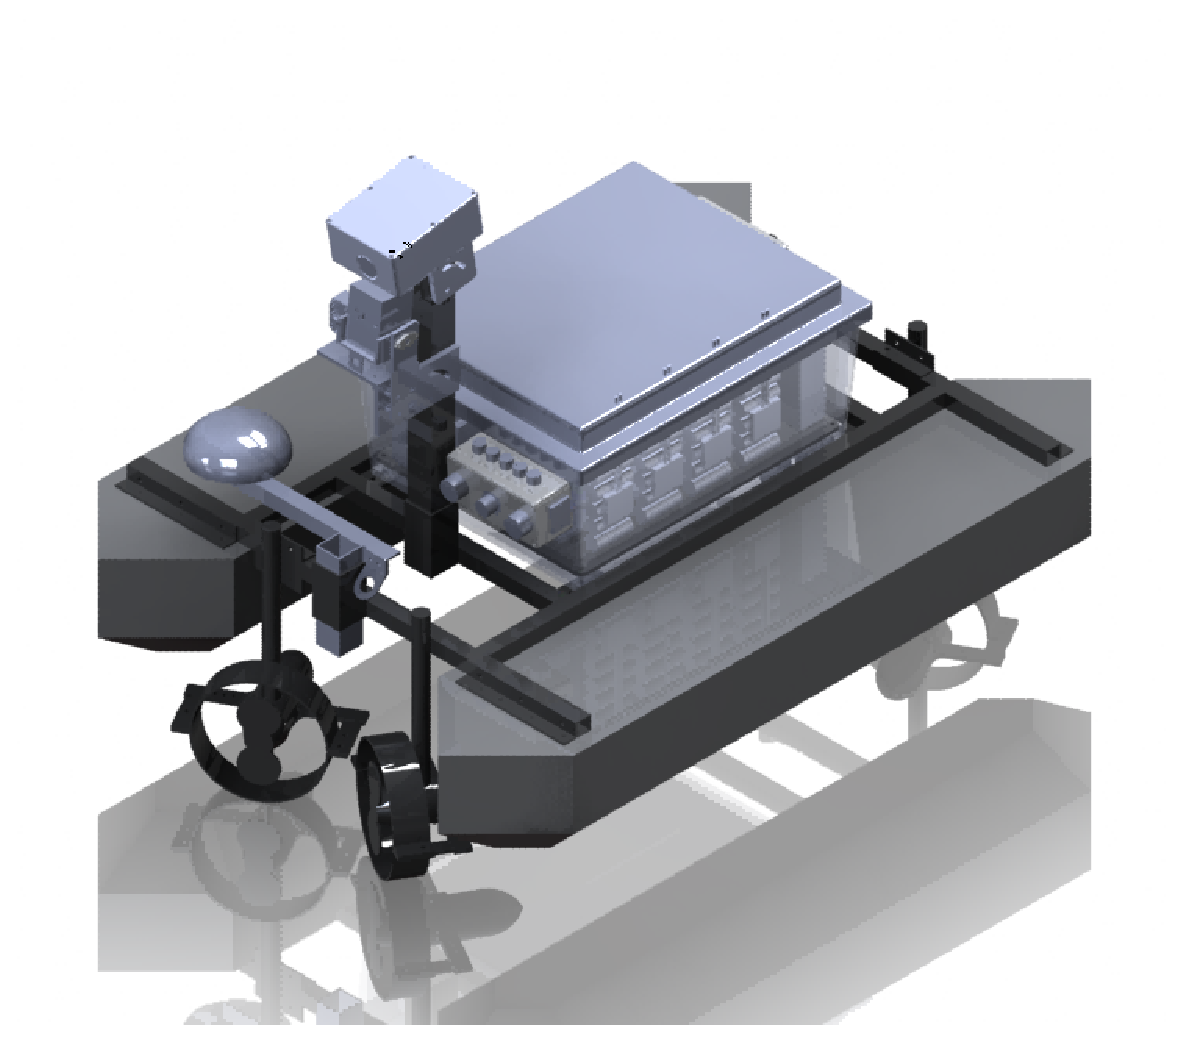
\includegraphics[width=3in]{whiterender}
\label{fig:pontoon}
\end{figure}



\begin{abstract}
The Robotics Club at UCF, with sponsorship from Army Research Labs (ARL) and the Institute for Simulation and Training (IST), presents a new platform for competing in AUVSI and ONR’s 5th international RoboBoat competition for 2012. Leveraging the knowledge from past competitions, the goal was to construct a platform that will be competitive in this year’s event, and ready to be improved upon by future UCF teams. A lightweight foam pontoon design reinforced with a polymer paint and a unique motor configuration allows for seamless movement in forward, reverse, rotation, and lateral directions. The electronics are mounted on modular DIN railing for reliability, ease of configuration and modification. Proven computer vision and mapping libraries from previous designs are extended to fuse multiple sensors including LIDAR, GPS, and compass for robust course navigation. A custom tilting servo mount was designed and fabricated for the LIDAR and heat sensor subsystem to enable 3D imaging of targets. The strategy this year was to give the vehicle the capability of accomplishing the four mandatory tasks (thrust test, start gate, speed gate, and buoy navigation) and three additional tasks (the cheaters hand, the hot suit, and the jackpot challenge).
\end{abstract}



\section{Introduction}
This year’s RoboBoat competition presents the team with several difficult challenges. With the input and experience from previous team leaders, the 2012 team decided to build a completely new vehicle.  Improvements to the boat include more simplified and reliable electronics and power regulation, enhanced fidelity and reliability of the motors, and lateral control. The pontoons were also redesigned for higher buoyancy and more stability while moving through the water. The electrical box received an upgrade which contains nearly double the volume over previous designs, implementing a cleaner and more modular interior.
 
An incremental design approach, following the spiral development process, lead to development of a sound platform. For example, hardware development stages included: requirements gathering and specification, 3D modeling, rapid prototypes, and final implementation. This process allows the early identification of gaps and design issues before final implementation reducing overall project risk and cost. The Gray Goose team focused on selection of hardware, sensors, and software to accomplish the challenges presented. The cheaters hand, the hot suit, and jackpot challenges are similar in that they require both computer vision and LIDAR sensors to locate targets. The boat includes a large water pump and nozzle mounted statically on the front of the boat for the cheaters hand, and a long range heat sensor mounted with the tilting lidar to complete the hot suit challenge. The camera is outfitted with a linear polarizer to cut down the glare from the water surface to detect the underwater buoy and an actuating arm is attached to allow button press for the jackpot challenge. Having accounted for future development, the new boat design leaves room on the frame for additional hardware for future teams to compete in new challenges.

An automated tilting LIDAR system that detects surfaces and buoys while actively scanning the surface of the water, the data is fused within advanced computer vision and mapping libraries proven at previous RoboBoat competitions. This combined data is used to identify and align with targets in the challenges. Computer vision is used to differentiate between colored buoys and start gates for the mandatory challenges. Buoys and other objects of interest are recorded in custom mapping software, called Cartographer, which handles path planning and obstacle avoidance. 

%%
% Mechanical
%%
\section{Mechanical Design}
One of the first decisions made when designing this craft was pontoon design and motor configuration. One of the goals for this year was to have reliable lateral control without complexity and points of failure. While lateral control is not strictly necessary for completing any of the challenges on the course, this additional ability improves performance in course correction and all target based challenges.  Several other improvements to the boat were made in terms of stability, weight and buoyancy of pontoons, as well as reliability and power of motors.

\subsection{Pontoons}
The most obvious modification to the pontoons was the removal of the keel. A keel-free design eliminates drag in the lateral direction, therefore a flat bottom pontoon was employed with angular geometry. The points at the front and the back of the pontoons are more blunt, decreasing rocking of the boat during rapid changes in direction. Also, the width of each pontoon was chosen so the boat will be more stable during lateral movement, and have less draft. A physics model implemented within SolidWorks was used to refine and test these design choices before construction of the final pontoons  and frame.

\begin{figure}[!h]
\centering
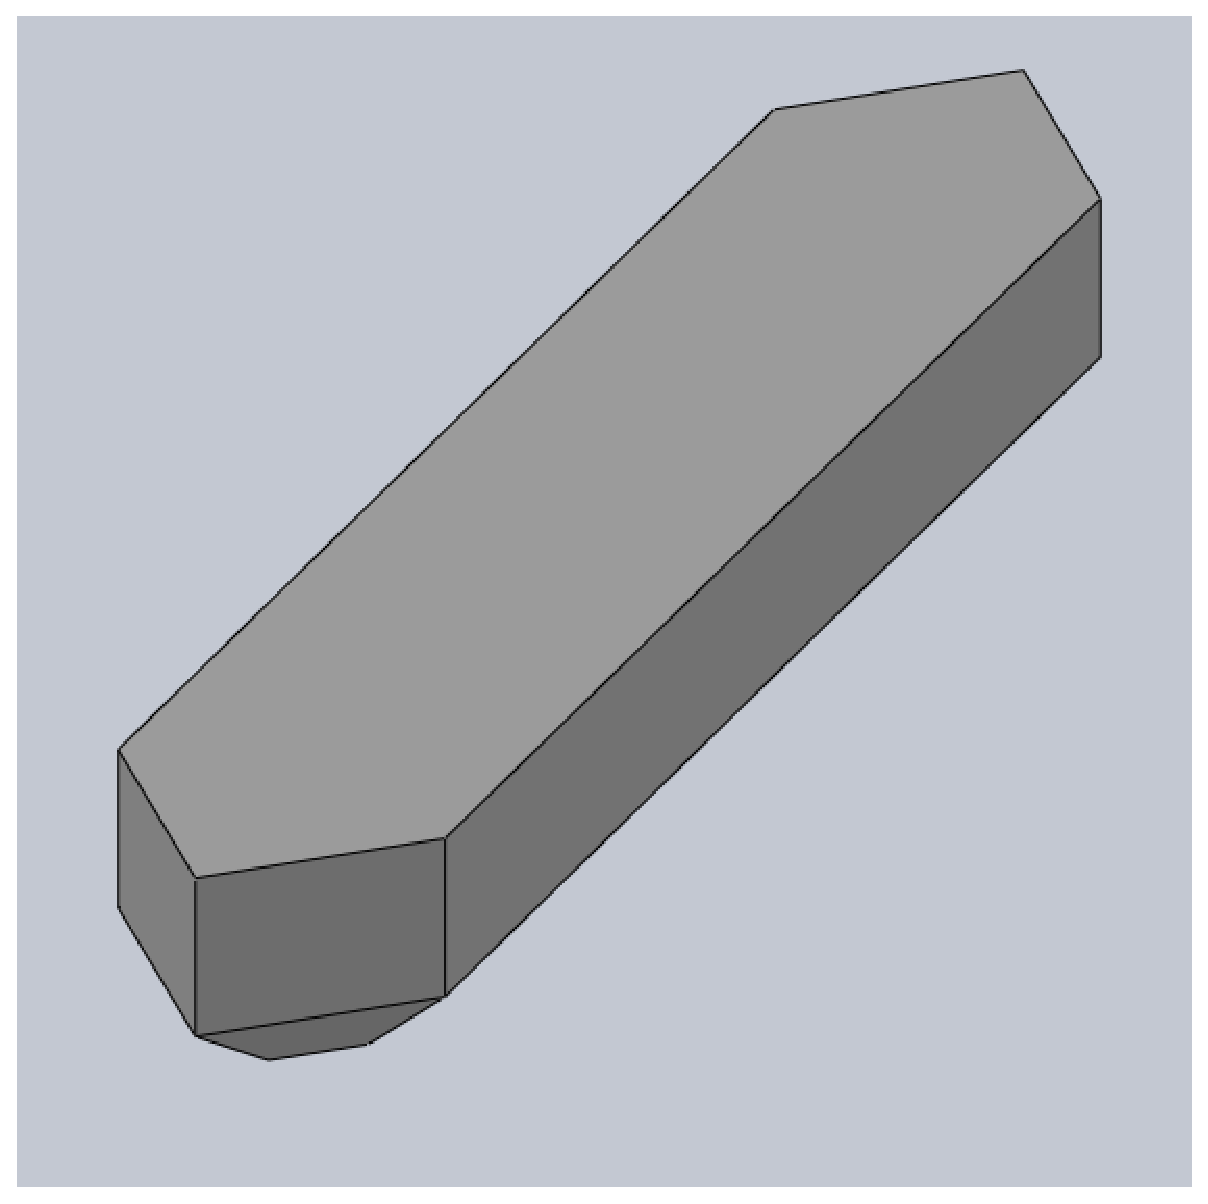
\includegraphics[width=2.5in]{images/pontoontrimetric}
\caption{3D render of pontoon design.}
\label{fig:pontoon}
\end{figure}

The pontoons were designed as a composite structure, and mostly fabricated in house. The bulk of each pontoon is white Styrofoam. The basic shape of the pontoon was professionally cut using a CNC hot knife. Polycarbonate plates with tapped holes for structural mounting are fitted and glued into insets cut into the front and back of each pontoon. The whole pontoon structure is covered with Styrospray 1000, a two part polyurethane coating approximately 0.03 inches thick. This adds an aesthetically appealing and rigid protective shell to the Styrofoam while retaining lightweight properties. Total weight of each completed pontoon is under seven pounds compared to last year’s which weighed over 12. This design was tested in the water, safely carrying up to a 140 pound load.

\begin{figure}[!h]
\centering
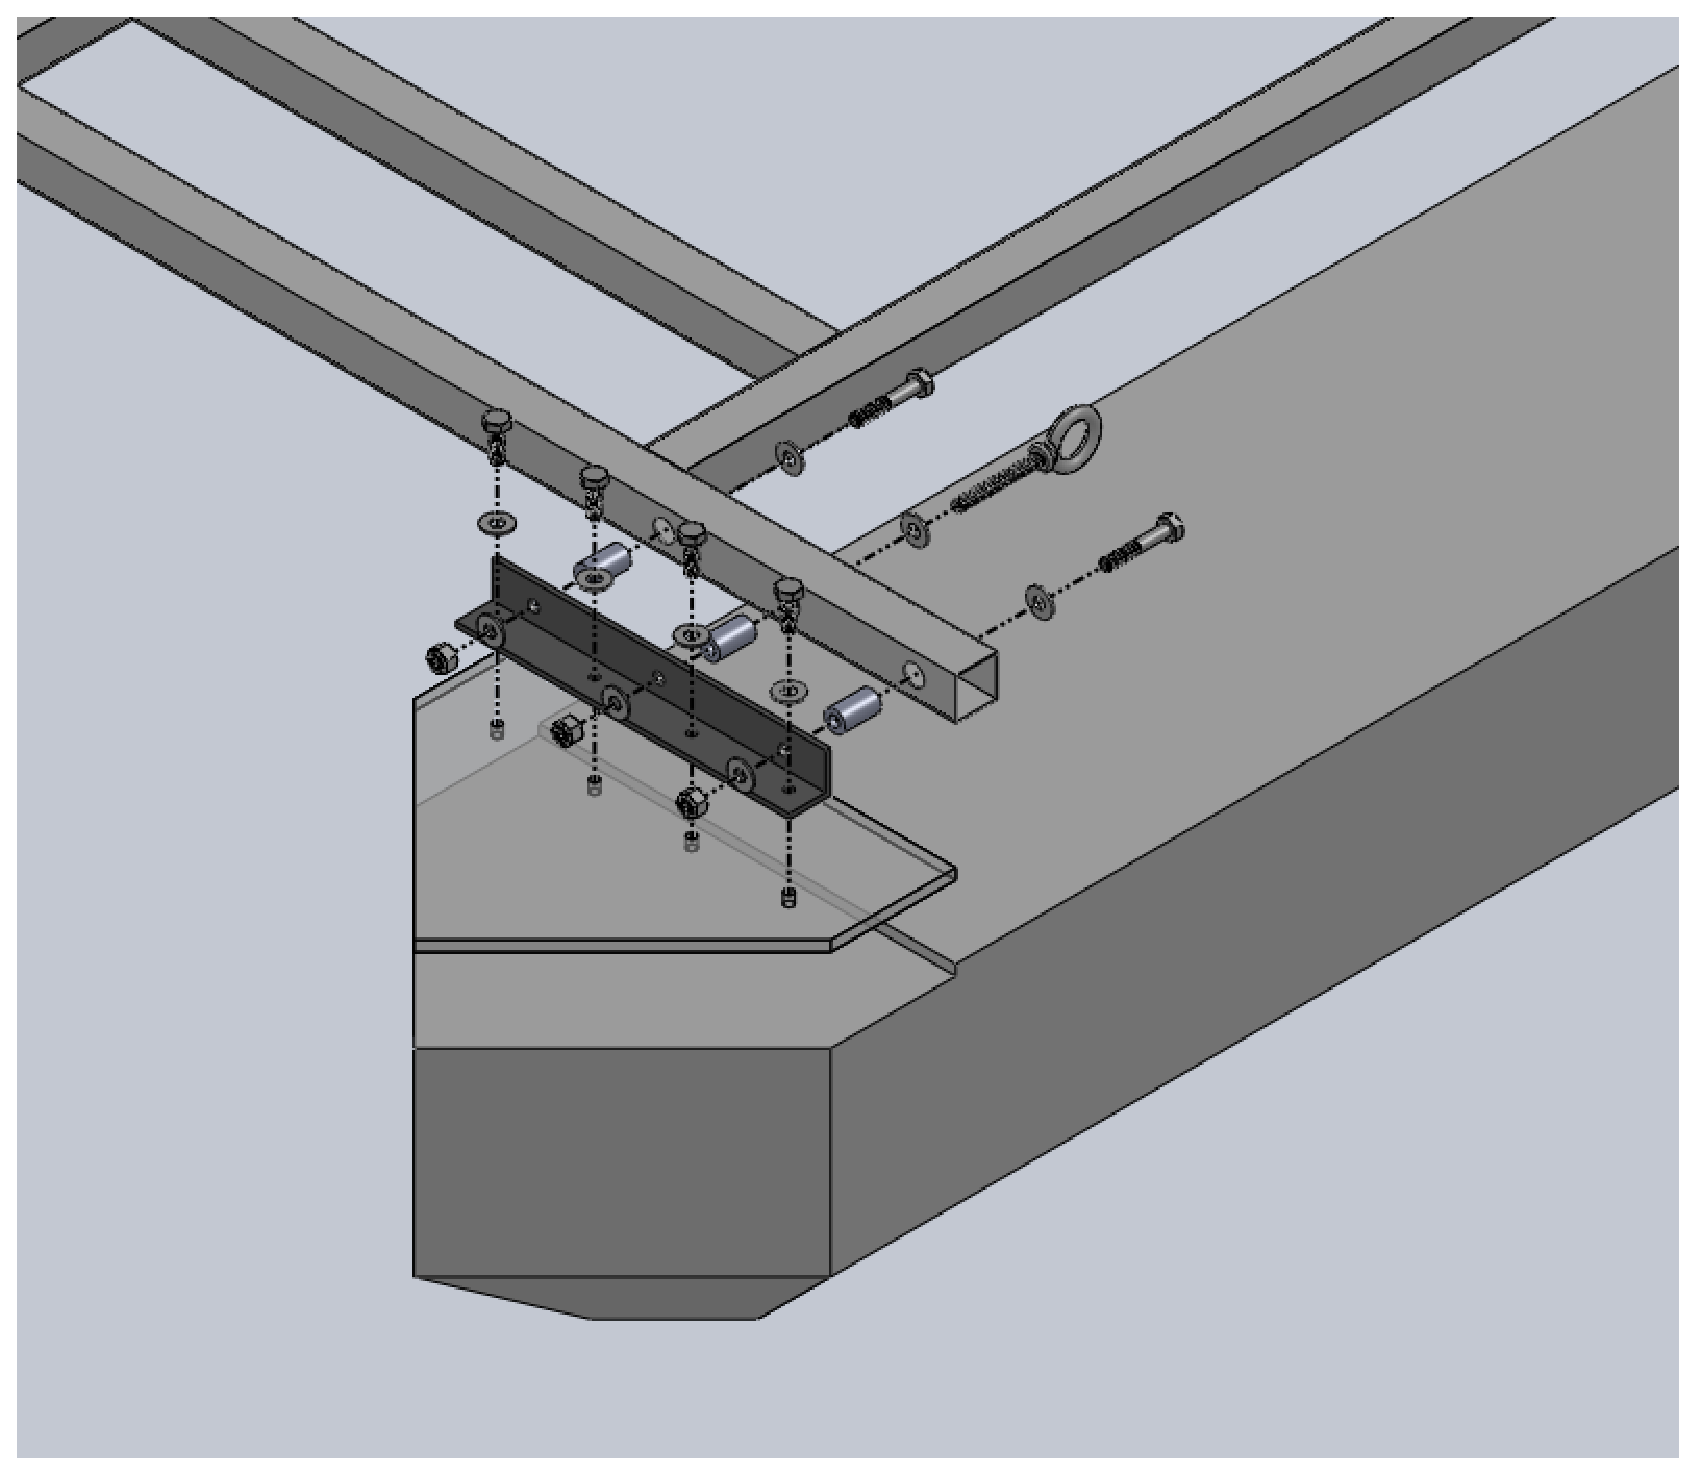
\includegraphics[width=2.5in]{images/pontoon-exploded}
\caption{Pontoon with polycarbonate mounting plate configuration}
\label{fig:pontoon-mount}
\end{figure}

\subsection{Frame}
A 1-inch square aluminum-tubing frame holds the two pontoons together. The frame was designed to have a dedicated section for the electronics box with five mounting locations to easily orient the center of mass at the center of the vehicle. The lengths of tube were cut on a horizontal band saw and professionally TIG welded together. The mounting plates for the electronics box and the L-channel were CNCed to ensure proper alignment. Holes drilled through the frame line up with the holes in the L-channel. Bolts hold the frame to the L-channel and the L-channel to the pontoons. Aluminum spacers reinforce areas of the frame with through bolts. One eyebolt is located on each mounting section to the pontoon for easy hoisting during water entry.

\begin{figure}[!h]
\centering
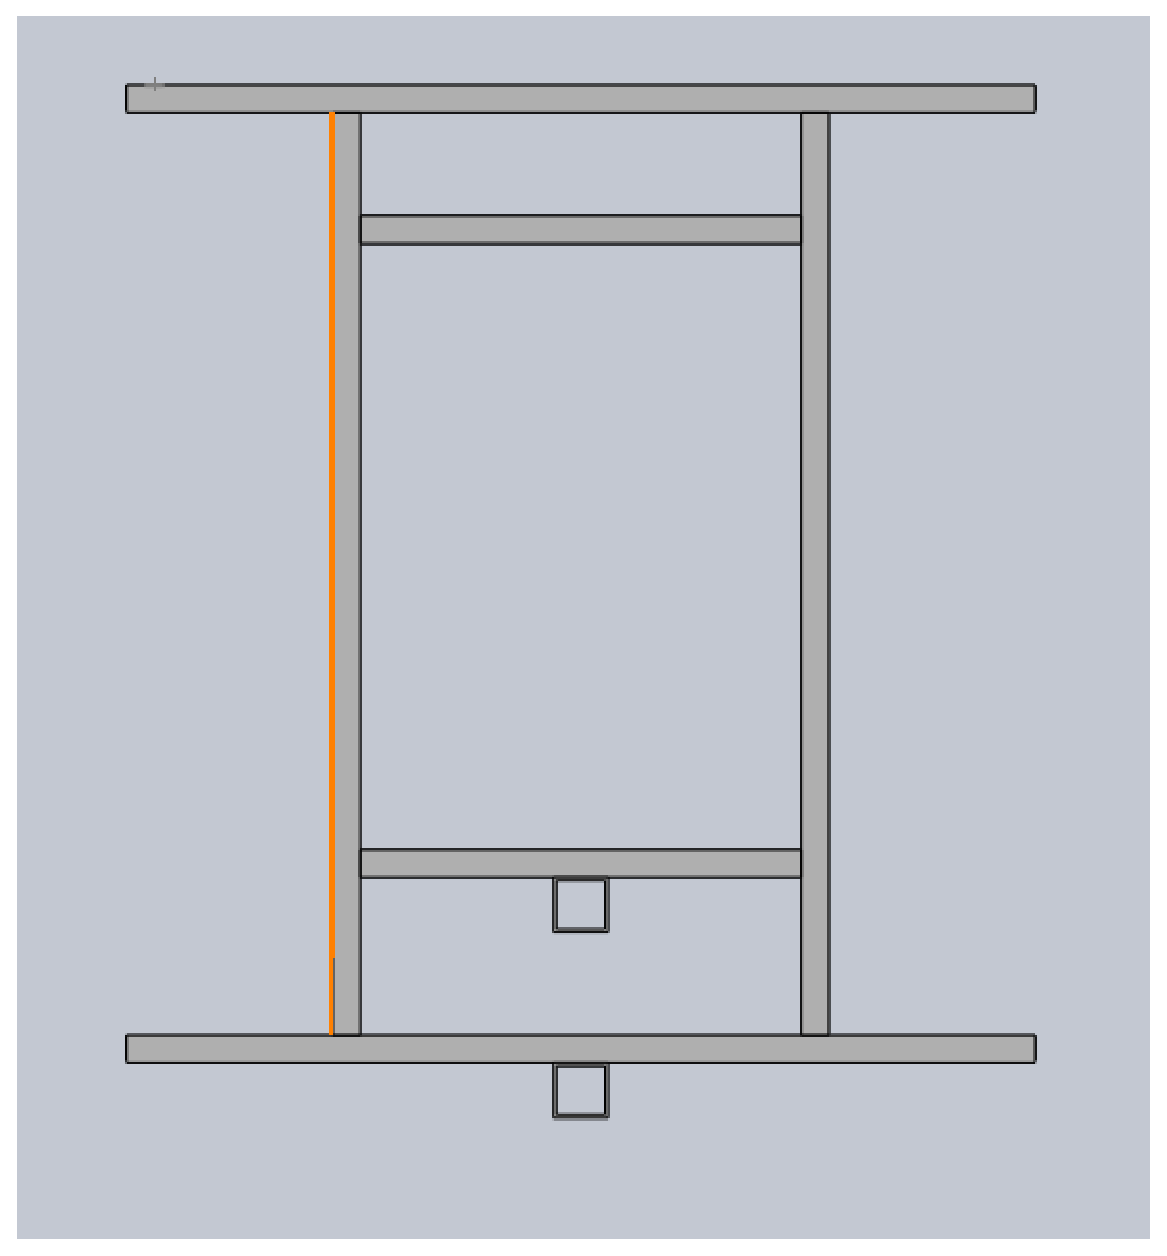
\includegraphics[width=2.5in]{images/topviewframe}
\caption{Top view of frame design.}
\label{fig:frame}
\end{figure}

\subsection{Motors}
The motor configuration is set up with a vector thrust design that easily allows the boat to move forward, backward, laterally, and spin in place with static motor mounts. This differs from previous designs which had one or more motors mounted to a rotating shaft that steered the boat for lateral motion. The previous design added complexity and reliability issues to lateral movement and ultimately ended up going unused. The new approach gains much more consistent mobility but loses some thrust in any direction, requires more motors (4) and increases power drain. The team felt these tradeoffs were worth the gains in additional maneuverability and reduced complexity. Bigger pontoons allow for greater weight capacity, so additional motor batteries added compensate for additional power loss.

The proof of concept of this design was tested using the platform of the previous year’s boat. With trolling motors attached to the old frame, several configurations were tested, including an X pattern, and Diamond pattern at various motor angles to verify results seen in simulation. The latter design was chosen because it was easier to control, perform lateral movements, and spin in place. Motor angles are rotated 30 degrees from forward, giving approximately a 33\% overall reduction in forward and reverse thrust, but adding 33\% thrust in the lateral direction.

\begin{figure}[!h]
\centering
\includegraphics[width=2.5in]{images/topviewmotorconfig}
\caption{Top view of motor configuration in final diamond pattern.}
\label{fig:frame}
\end{figure}

Previous UCF teams had malfunctions with Seabotix and CrustCrawler motors which hindered their performance at competition. This year, consumer trolling motors were selected for a more reliable product. This motor selection added several challenges which were overcome with some engineering and creativity. To make the motors more appropriate for a robotic vehicle, they were cut down and refitted for use with the robot’s electronics box. Motor shrouds were not available off the shelf and needed to be custom designed and fabricated. 

\begin{figure}[!h]
\centering
\includegraphics[width=3in]{images/motor-beforeafter}
\caption{Before and after modifications to trolling motor.}
\label{fig:frame}
\end{figure}

\subsection{Mast and Sensor Mounts}
The sensor mast hosts the camera, LIDAR, and temperature sensor. At the top of the mast sits the camera box, designed to sit the camera exactly in the center of the vehicle. The mount allows for 60 degrees of rotational freedom for vantage angle and can easily be modified manually.
Sitting just below the camera is the LIDAR and IR temperature sensor mount. This mount is designed to host each in the center of the vehicle. A stationary mounting plate with 60 degrees of rotational freedom is attached to the mast. On top of that mount is an electronically controlled platform that tilts the sensors to gain a 3D map and temperature profile for the cheater’s hand challenge.

%%
% Electrical
%%
\section{Electrical Design}
The electronics of this year’s ASV was redesigned to improve on previous year’s shortcomings. Issues that were resolved include: unreliable motors, power inefficiencies, and non-modular layout. The team first identified the problems, brainstormed and researched solutions, established design requirements, prototyped and finalised the best design ultimately producing a final board. 

\subsection{Propulsion}
 Last year’s motor selection of Crust Crawlers proved to be unreliable and inefficient. This year, research was done to find options and choose a vetted off the shelf technology, the trolling motor. This motor type is proven to perform in the marine environment, being installed on many consumer watercraft. A 12 volt rated system was selected based on the availability, affordability, and desired specifications on thrust, form factor, and controllability. The vertical tiller of the trolling motor housed the wires and allowed for mounting to the vehicle’s frame. Once motors were purchased, a power/thrust test was done. Each motor has up to 13 pounds of thrust in the forward direction at 13 amps, and nearly 11 pounds at 13 amps in reverse.
 
\begin{figure}[!h]
\centering
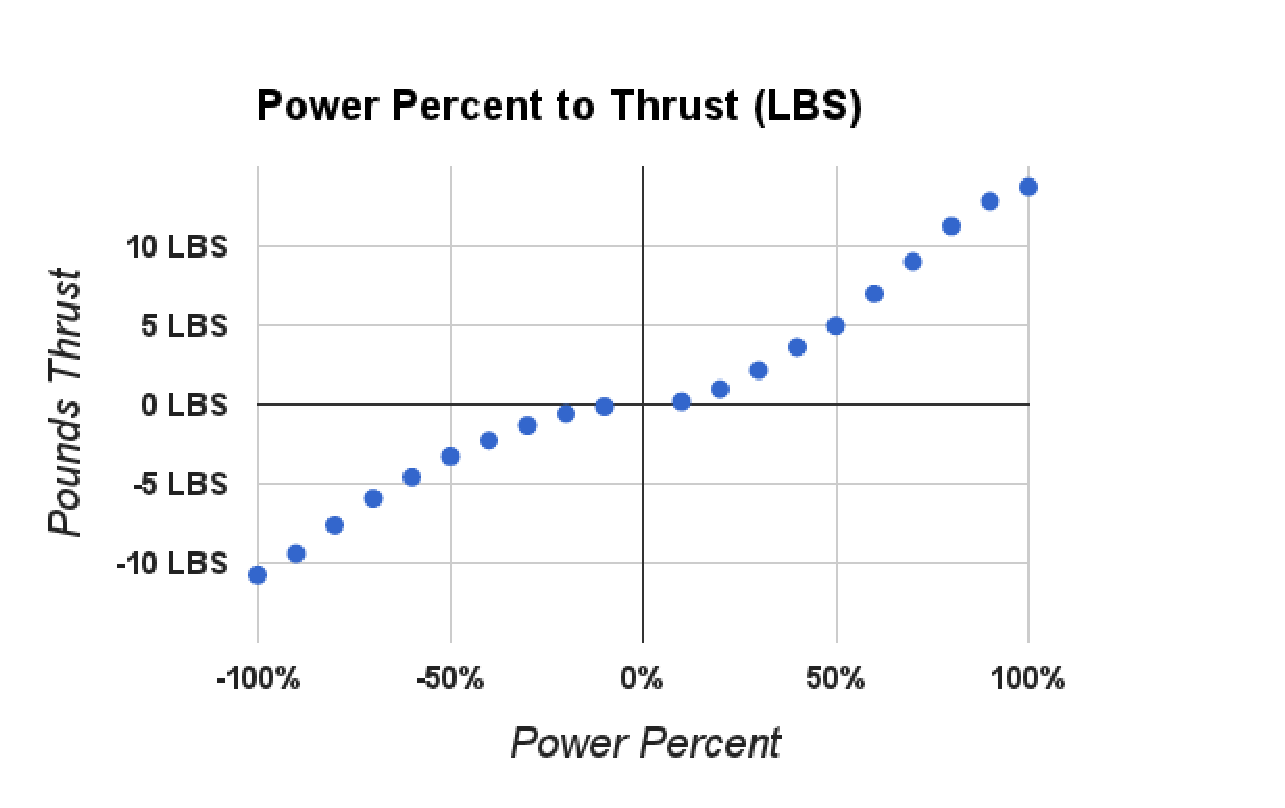
\includegraphics[width=3in]{images/powerthrustchart}
\caption{Thrust chart showing LBS thrust. 100 percent was approximately 13 amps in forward and reverse. Thrust sampled at 10 percent intervals.}
\label{fig:powerthrustchart}
\end{figure}

\subsection{Batteries}
A dual power source configuration is incorporated, separating motor and logic power sources. Power isolation has two benefits: preventing interference between systems and allowing for an emergency cut-off of power to actuating devices in off-normal situations. The motors are powered from 4-cell LiFePO4 batteries providing nominal 12.8V, within motor and motor controller requirements. Additional motor batteries are placed in parallel to extend the runtime of the vehicle, with a total capacity of 26.4Ah (approximate runtime of 4 hours). The logic components of the vehicle (e.g. onboard computer) are powered from 6-cell Li-Po batteries providing nominal 22.2V. This higher voltage power rail more efficiently delivers power to all devices. A high-efficiency switching voltage regulator provides a regulated 12V power source required to operate various sensors and devices.

\subsection{Printed Circuit Board}
A custom printed circuit board (PCB) was designed and fabricated to integrate analog and digital signals for this year’s vehicle and provide new student members an opportunity to learn PCB design. The PCB contains an ARM based PSoC3 microcontroller that handles several responsibilities:
\begin{itemize}
\item Interprets RC Receiver Signals
\item Commands motor controllers
\item Monitors vehicle status (Battery voltages, temperature, etc.)
\item General Purpose Input Output (GPIO)
\item High Current Outputs
\item USB-to-Serial Interface to Computer
\end{itemize}

\begin{figure}[!h]
\centering
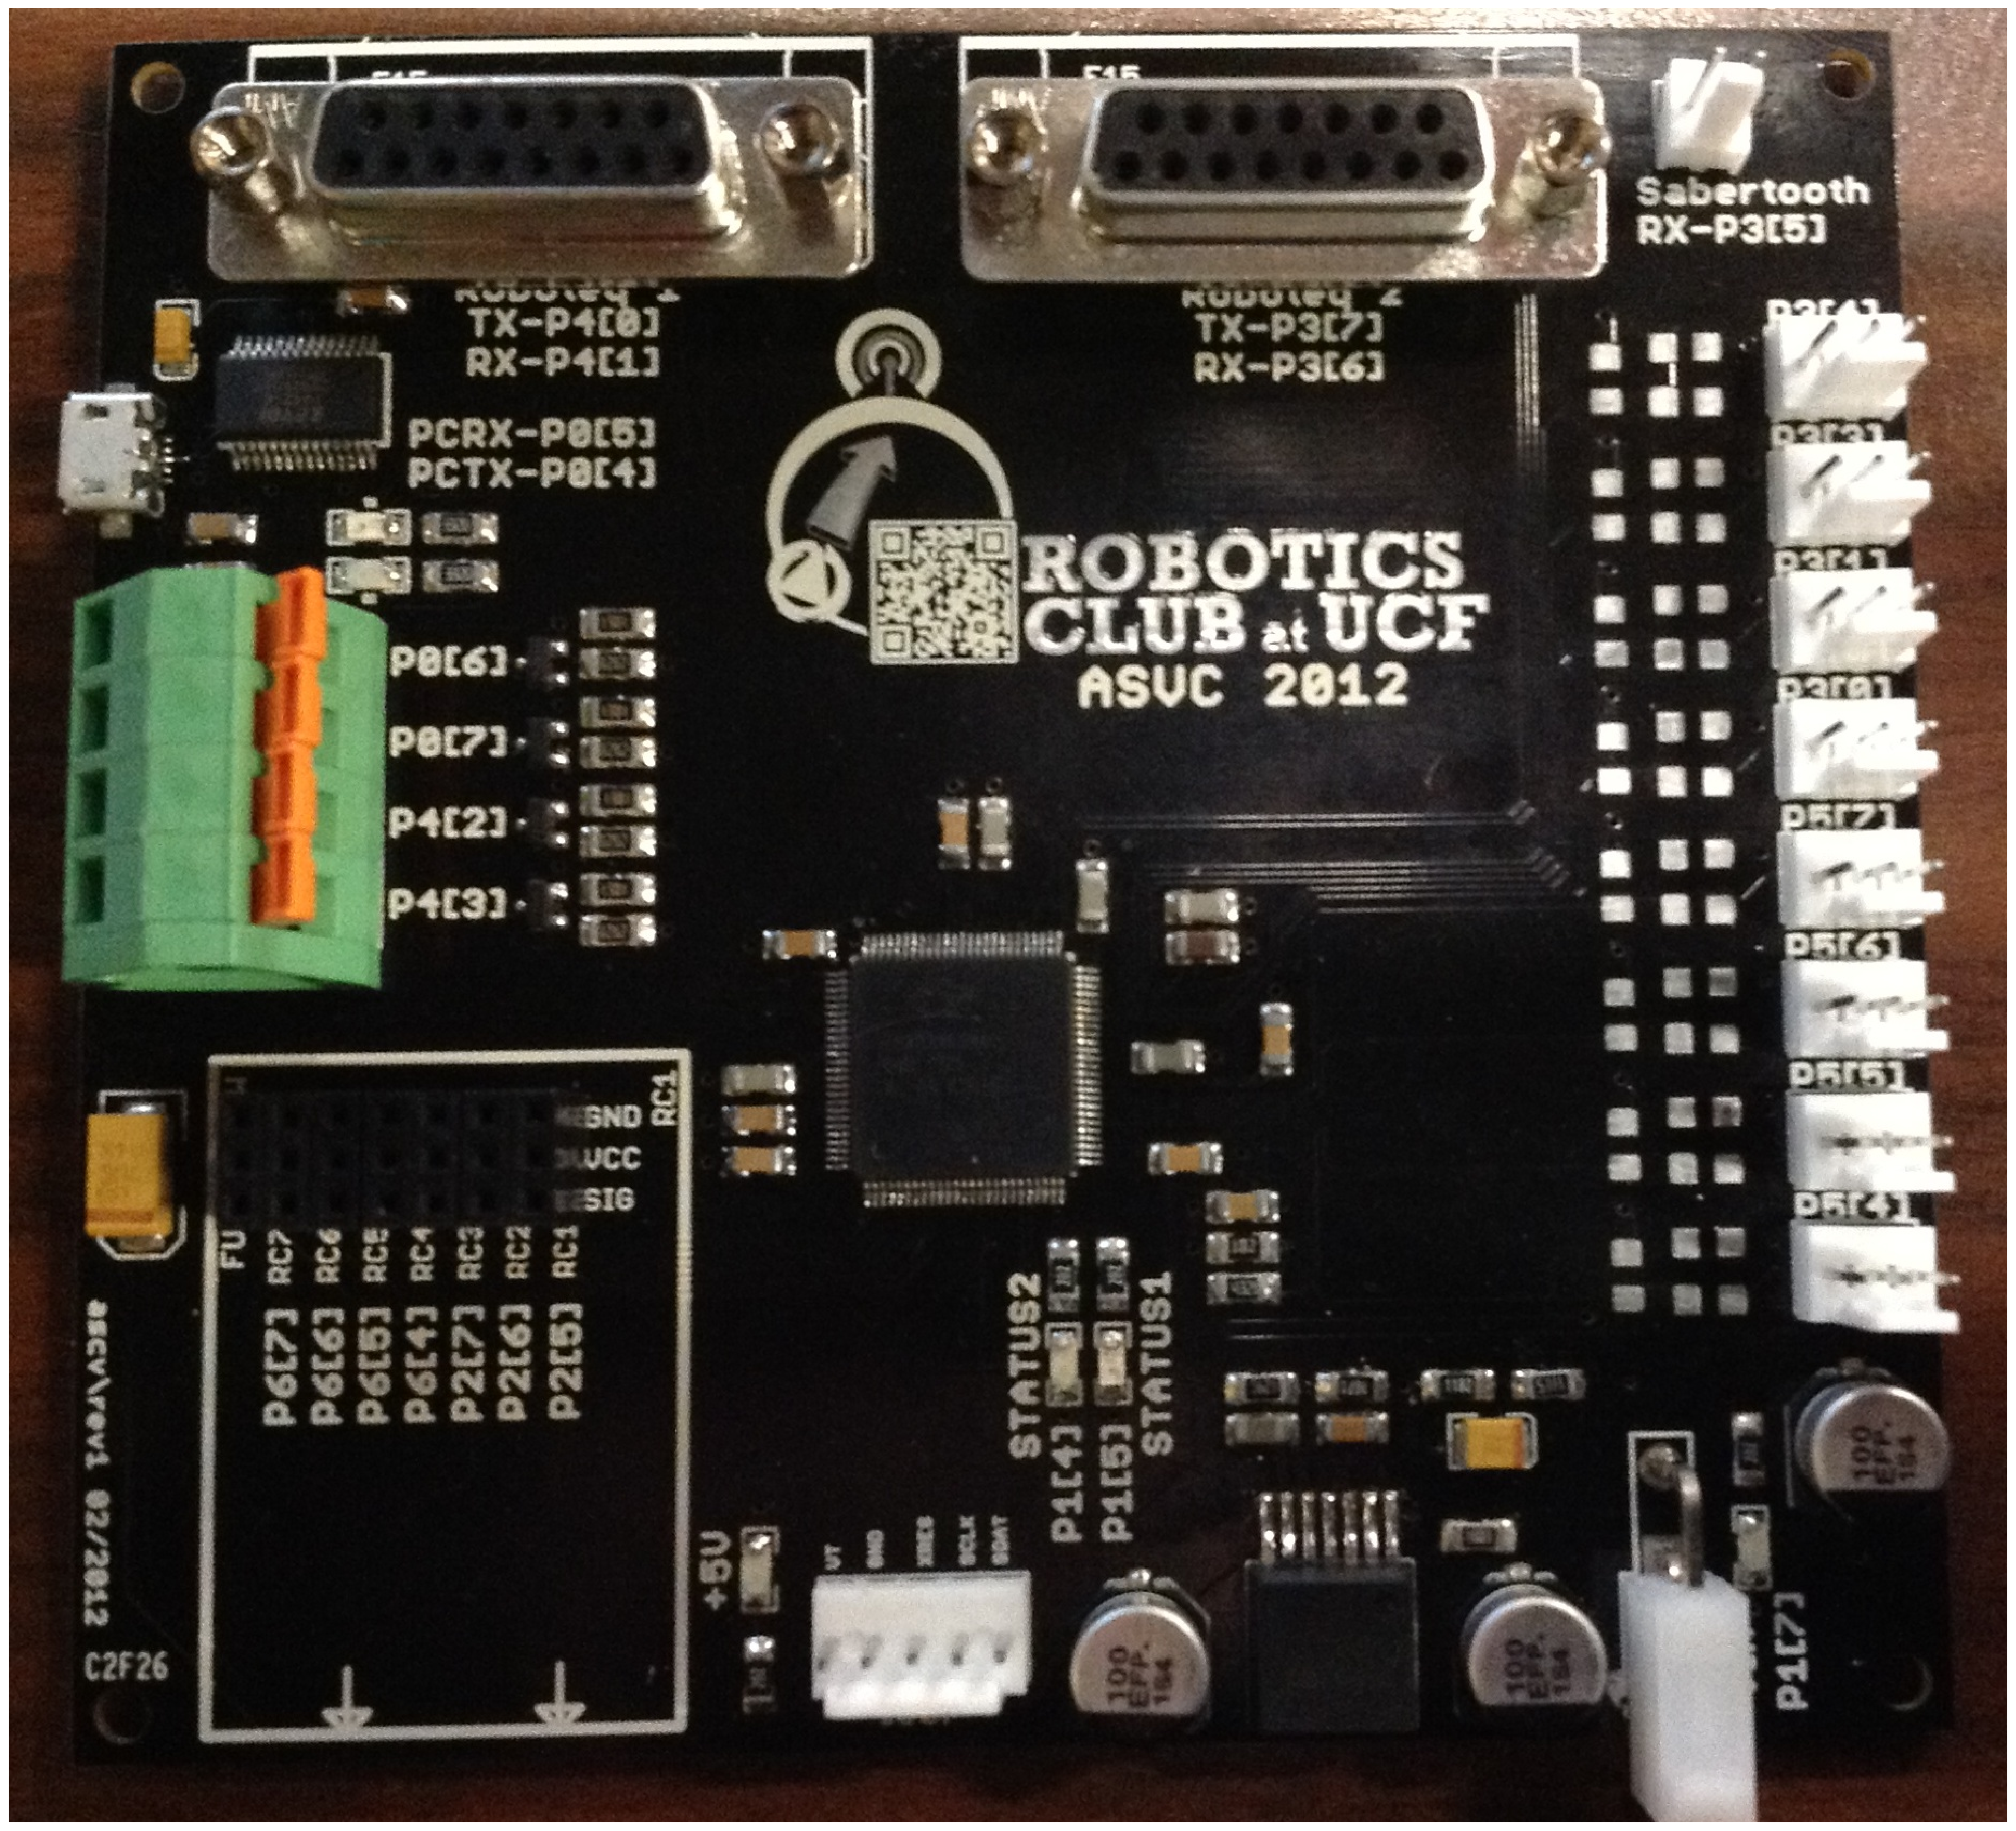
\includegraphics[width=3in]{images/pcb-picture}
\caption{Final Custom PCB}
\label{fig:pcb-real}
\end{figure}


The high current outputs on the PCB allows the microcontroller output pin that is limited to 5mA is able to switch the low-side (ground) through a high power mosfet of 1A. This is utilized on the vehicle to switch high current components including the autonomous indicator strobe light and low battery audible indicator. Commercial connectors on the board interconnect various components and allow for expandable future uses.

\subsection{Wireless Networking}
A high power wireless networking solution provides software developers the ability to debug the vehicle’s programming remotely. This ability is a key factor in efficient use of testing time on the course, supporting remote configuration and adjustment of parameters on the fly for optimization. Previous designs utilized standard IEEE 802.11b/g/n network wireless routers to maintain a remote connection, which proved to be unreliable at distances achieved across the entirety of the lake. Ubiquiti Networks airMAX Rocket M wireless base station is a powerful 2x2 MIMO modem that has incredible range, speed and ultimate RF performance in outdoor environments. The network is configured as a point-to-point seamless link, bridging the vehicle and operator command center’s network.

\subsection{Power Distribution}
Power distribution is achieved through the use of an industry standard DIN rail. Chosen for its modularity and standardisation of parts, the DIN rail provides a solid mounting point for high current devices. Out of the water power (i.e. shore power) is delivered through the use of a PC-6 connector wired to a 120 volt AC power supply providing 24 volts at 15 amps. A shore power relay, triggered by the AC current itself, switches from battery power to the power supply. This effectively replaces the batteries with the power supply when an AC current is supplied for additional testing and development when not in the water.

\begin{figure}[!h]
\centering
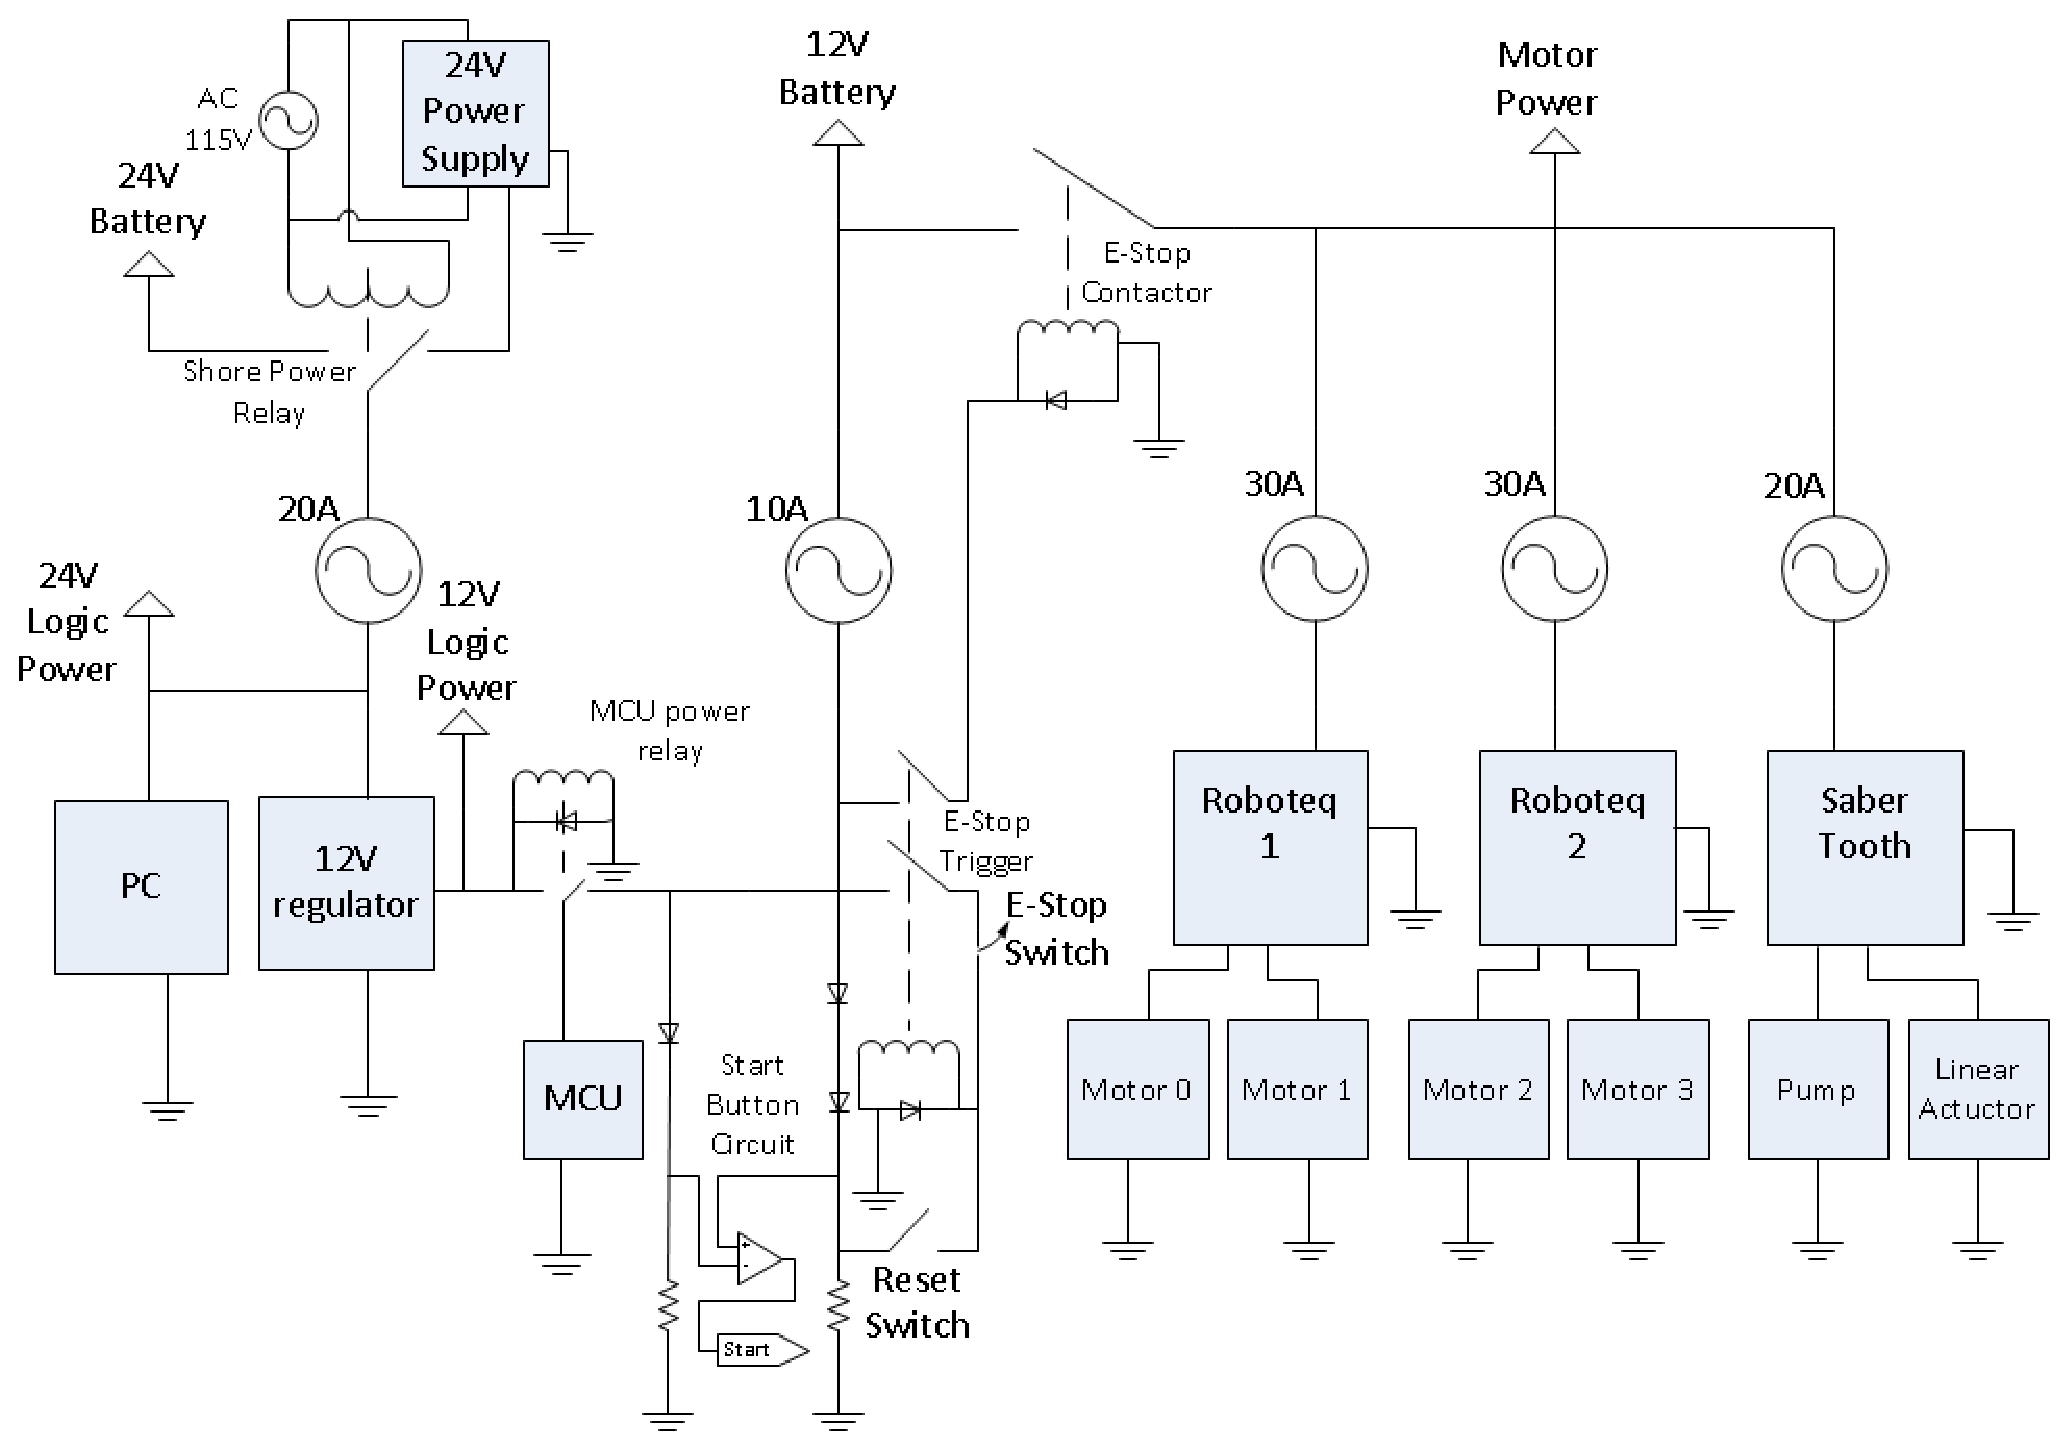
\includegraphics[width=3in]{images/powerdiagram}
\caption{Power Diagram}
\label{fig:powerdiagram}
\end{figure}

\subsection{Emergency Stop}
Safety is addressed with the implementation of an emergency stop circuit achieved using a 200 amp 12 volt coil contactor triggered by a single pole double throw relay. One of the throws of the trigger relay triggers the contactor and the other is used to control the relay itself. A normally closed emergency stop switch is used to cut off the power to the trigger relay, and a normally open reset switch is used to re-energise the trigger coil. To improve simplicity, a circuit was added to use the reset switch as an initial start switch for the transition into autonomous mode. This circuit uses a diode drop as a reference and a double diode as a trigger. The double diode is initially acknowledged when the switch is open, and set to an equipotential when the reset switch is pressed. The data read from the double diode and the reference diode is passed to a comparator in the microcontroller, and is seen as a 1 when the switch is pressed an 0 when the switch is idle. 

\subsection{Temperature Sensor}
Completing the hot suit challenge requires the addition of an infrared temperature sensor to obtain the temperature values of the four signs. Finding a sensor responsive enough for the range required to complete the task proved difficult, but the team decided on a Raytek MI Series infrared temperature sensor. The sensor has a fresnel lens with 22:1 distance to spot optics and an eight to fourteen micrometer spectral range which enables the boat to obtain accurate temperature measurements in the infrared light spectrum. This accuracy allows the boat to sit roughly 22 feet away from the signs for the task and still accurately distinguish which suit is hot. The range of input voltages, output configurations, and the IP65 housing of the Raytek sensor fit in perfectly with the electrical designs that were in place and proved to be very reliable in even the worst weather conditions.

%%
% Software
%%
\section{Software Design}
The software this year heavily utilizes the infrastructure built on from previous teams. This software has shown to be proficient in completing the start gate, speed gate, and buoy navigation challenges using color finding. The new boat configuration includes important changes in computer vision (CV), artificial intelligence (AI), and motor control system enabling greater capabilities over past implementations. AI, vision, control and sensor integration are done on a quad core mobile intel processor with 8GB of RAM.

\subsection{Architecture}
The robot’s underlying software architecture is very similar to last year’s boat, and is fairly standard across all Robotics Club at UCF vehicles. Sensor control and communication is routed through the Joint Architecture for Unmanned Systems (JAUS) standard using an open source implementation called JAUS++.  Sensor data is packed in JAUS messages and subscribed to by the AI program, which evaluates and acts on the data. This modular approach has several advantages, the biggest being easy reuse across completely different platforms, such as the underwater, ground vehicle, and boat due to the hardware independence of JAUS.  On the boat, an always on program maintains connections and communication to all hardware devices, while a separate AI program can be started, stopped, and reconfigured without the need to reconnect to sensors. Using the message passing framework provided by JAUS, software located on other network computers can subscribe to sensor data and take hardware control for fast testing and development.  The software architecture implementation also includes logging of all data generated by sensors. This information can be played back within a simulation sandbox or evaluating AI behavior on recorded data. This powerful feature enables fast debugging of robot decision making in addition to development of new AI modules without the need to physically operate the robot.

\subsection{Motor Control}
The unique motor configuration of the Gray Goose allows seamless movement in any direction on the water. This configuration affords power and agility without sacrificing the fine movement needed for achieving this year's tasks. Reliable and smooth lateral control can now be used for advanced maneuvers around targets and through buoy channels. Rotational speed has also been improved thanks to the symmetrical diamond configuration of the motors.

The AI now has access to maneuvers such as face a target while moving around it, align to target angle, and lateral search as opposed to traditional left/right sweeping searches. These new capabilities support lining up to targets without losing them from sensor view. Commands such as move to GPS waypoint, maintain velocity, and heading commands are carried over from last year’s robot. High level waypoint commands are translated to velocity commands and then to thrust commands in three channels (linear x, linear y and rotational z). Velocity is estimated by GPS data combined from both the GX3 and Navcom sensors. Thrust output is determined by individually tuned PID controllers for rotation and linear velocities. 

\begin{figure}[!h]
\centering
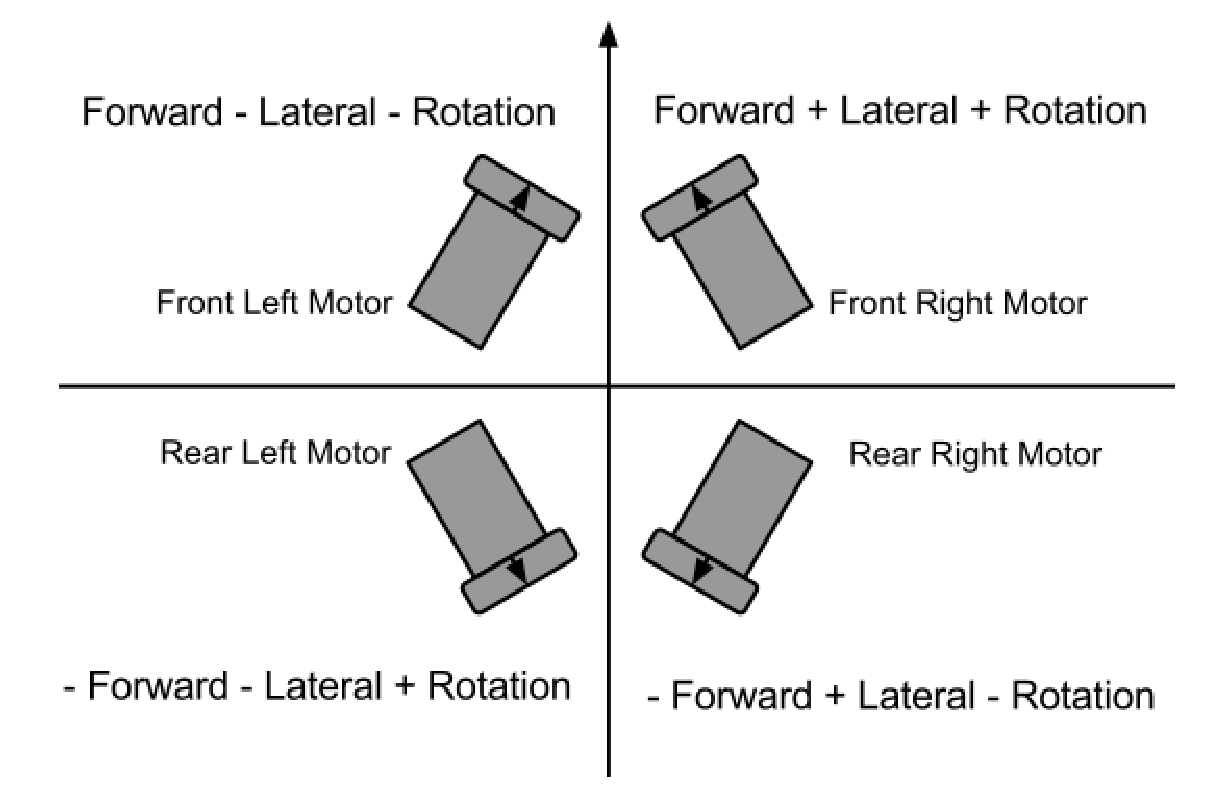
\includegraphics[width=3in]{images/motorconfigsoftware}
\caption{This shows 3 channel mixing to 4 motors in a diamond configuration. Each quadrant contains a unique combination of channels.}
\label{fig:motorconfigsoftware}
\end{figure}

Low level motor control requires mixing three channel movement commands to four motors. Symmetrical positioning of motors simplifies the mathematics needed for this process. Each motor can be placed in a quadrant where each quadrant is a unique linear combination of the three channels.

\subsection{Computer Vision}
A Basler camera delivers high resolution imagery and frame rates at the expense of slightly higher CPU usage for capture. The camera lense provides 120 degree field of view (FOV) with minimal distortion. Clear, high resolution images and high FOV support object spotting through color segmenting at near and far distances, making buoy navigation safer. All vision processing is done in C++ using the OpenCV library.


\subsection{State Machine}
The course is broken down into missions, one for each challenge. Each mission can be broken down further into states and sub-states, in which discrete actions are taken based on fused sensor data. When certain conditions are met, states will transition to new states until an end state is reached and/or the mission is complete. Each mission has a time-out value which ensures the vehicle can “give up” and move on to the next mission maximizing challenges attempted. 

\begin{figure}[!h]
\centering
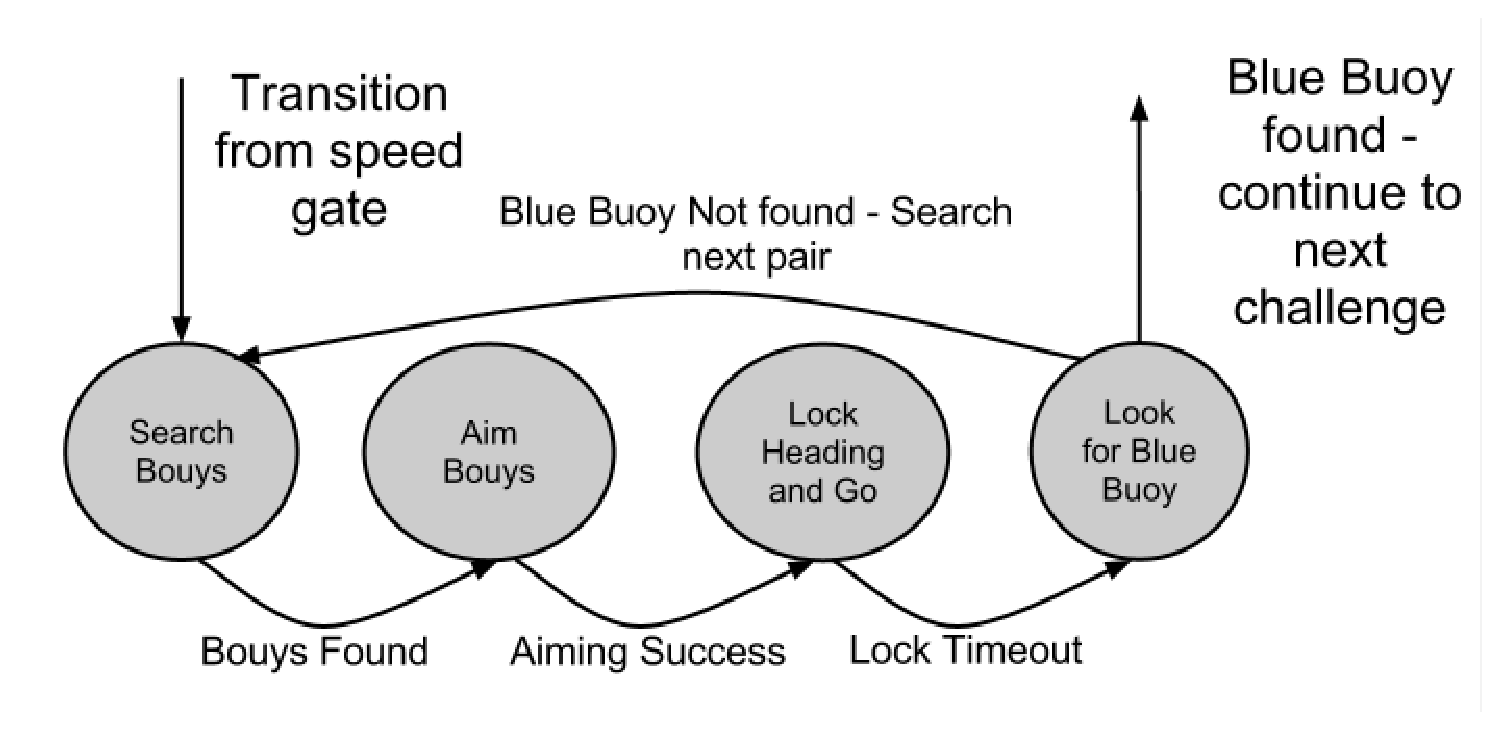
\includegraphics[width=3in]{images/statemachinediagram}
\caption{A simplified state machine diagram showing possible buoy navigation logic.}
\label{fig:statemachinediagram}
\end{figure}

\subsection{Point Cloud}
This year the boat has an important new addition to its sensor package. A tilting Hokuyo LIDAR and Dynamixel servo allows laser data to be added to a 3D point cloud  used in conjunction with computer vision to better acquire targets of interest. As the LIDAR pivots, angle values are read from the Dynamixel and points are translated and input into the open source Point Cloud Library (PCL).  The 3D point cloud is calibrated to camera data to enhance color segmentation and reduce false positive detection. Aiming water cannon temperature gun and button press arm rely on range finding, coupled with computer vision to identify the correct target.

\begin{figure}[!h]
\centering
\includegraphics[width=3in]{images/3dlidarfront}
\caption{An example of 3D data collected from tilting lidar taken from inside the lab. Distances have been color coded into a heat map. }
\label{fig:3dlidarfront}
\end{figure}

\section{Expenses}
Our expenses can be found in Table~\ref{tbl:expense}


\section{Conclusion}
The Robotics Club at UCF has been hard at work on a completely new Autonomous Surface Vehicle (ASV) called the Gray Goose. Innovative new features such as a vector thrust control for three degrees of movement on water, wider, more stable and lightweight pontoons, point cloud generation with a tilting Hokuyo LIDAR and improved power regulation will allow the vehicle to go far in this year’s competition.


\section*{Acknowledgment}
The team would like to thank our sponsors at Army Research Labs (ARL) Simulation and Training Technology Center (STTC), the University of Central Florida’s (UCF) Institute for Simulation and Training (IST), along with our faculty advisor, Daniel Barber at IST, industry advisor Dr. Gary Stein at Primal Innovation, Irwin Hudson at ARL and Dennis Coleman at the UCF Machine Lab for letting us use their equipment.

\begin{table*}[!h]
%\renewcommand{\arraystretch}{1.3}
% if using array.sty, it might be a good idea to tweak the value of
% \extrarowheight as needed to properly center the text within the cells
\caption{Expenses}
\label{tbl:expense}
\centering
% Some packages, such as MDW tools, offer better commands for making tables
% than the plain LaTeX2e tabular which is used here.
\begin{tabular}{|c|c|c|c|c||c|}
\hline
\bfseries Purpose & \bfseries Type & \bfseries Units & \bfseries Source & \bfseries Cost Per& \bfseries Total\\
\hline\hline
Camera & Basler acA1300-30gc Gig-E Camera & 1 & Robotics Club & 700 & 700\\
\hline
Lense & 135 Degree C Type Lense & 1 & Previous Year & 500 & 500\\
\hline
Motors & Sevylor Trolling Motor SBM18 & 7 (4 + 3 spare) & Robotics Club & 100 & 700\\
\hline
LIDAR & Hokuyo UTM30LX & 1 & Sponsorship & 5500 & 5500\\
\hline
Tilt Servo & Dynamixel RX45 & 1 & Previous Year & 50 & 50\\
\hline
Differential GPS & Navcom NCT-2030M & 1 & Sponsorship & 5000 & 5000\\
\hline
Compass, Aux GPS & Microstrain 3DM GX3 - 45 & 1 & Sponsorship & 3800 & 3800\\
\hline
Computer & Custom Mini ITX Intel Quad Core & 1 & Previous Year & 1000 & 1000\\
\hline
Pontoons & Custom foam carved, reinforced, painted & 2 & Robotics Club & 100 & 200\\
\hline
Frame & Custom aircraft grade welding & 1 & Robotics Club & 150 & 150\\
\hline
Logic Batteries & Thunderpower Pro lite v6 22.2V LiPo 5.5Ah  & 4 & Sponsorship & 200 & 800\\
\hline
Motor Batteries & Powerizer 12.8V LiFePO4 6.6Ah & 4 & Previous Year & 75 & 300\\
\hline
Motor Controller & Roboteq SDC2130 & 2 & Robotics Club & 175 & 350\\
\hline
Aux Motor Control & Sabertooth dual 12A motor driver & 1 & Previous Year & 75 & 75\\
\hline
Electronics Box & Allied Molded AM2068RT & 1 & Robotics Club & 180 & 180\\
\hline
Connectors/Wiring & Misc wires and connectors & - & Robotics Club & 400 & 400\\
\hline
Pump & Sureflo Bilge Pump 4700 GPH 12v 16A & 1 & Robotics Club & 100 & 100\\
\hline
Power Supply & Rhino PSM24-360S & 1 & Robotics Club & 250 & 250\\
\hline
Power Distribution & DIN Rail and Modular Components & - & Robotics Club & 600 & 600\\
\hline
Microcontroller  & Custom PCB and PSOCK & 2 & Robotics Club & 75 & 150\\
\hline
Heat Sensor & Raytek MI Series 22:1 Thermal Sensor & 1 & Robotics Club & 130 & 130\\
\hline
Misc Parts & Lights, Boxes,Materials, etc & - & Robotics Club & 1000 & 1000\\
\hline
Long Range Wifi Antenna & 5GHz AirMax Dual Omni, 10dBi & 2 & Sponsorship & 125 & 250\\
\hline
Short Range Wifi Bridge & Linksys WGA600N Wireless N Gaming Adapter & 1 & Previous Year & 50 & 50\\
\hline
Long Range Wifi AP & RocketM5 802.11N MIMO 5 GHz Rocket AP & 2 & Sponsorship & 90 & 180\\
\hline
&&&&\bfseries Total & 21615\\
\hline
\end{tabular}
\end{table*}

% that's all folks
\end{document}

